 %%%%%%%%%%%%%%%%%%%%%%%%%%%%%%%%%%%%%%%
 % Wenneker Resume/CV
 % LaTeX Template
 % Version 1.1 (19/6/2016)
 %
 % This template has been downloaded from:
 % http://www.LaTeXTemplates.com
 %
 % Original author:
 % Frits Wenneker (http://www.howtotex.com) with extensive modifications by 
 % Vel (vel@LaTeXTemplates.com)
 %
 % License:
 % CC BY-NC-SA 3.0 (http://creativecommons.org/licenses/by-nc-sa/3.0/
 %
 %%%%%%%%%%%%%%%%%%%%%%%%%%%%%%%%%%%%%%
 
 %----------------------------------------------------------------------------------------
 %	PACKAGES AND OTHER DOCUMENT CONFIGURATIONS
 %----------------------------------------------------------------------------------------
 
 \documentclass[a4paper,12pt]{memoir} % Font and paper size
 
 %%%%%%%%%%%%%%%%%%%%%%%%%%%%%%%%%%%%%%%%%
% Wenneker Resume/CV
% Structure Specification File
% Version 1.1 (19/6/2016)
%
% This file has been downloaded from:
% http://www.LaTeXTemplates.com
%
% Original author:
% Frits Wenneker (http://www.howtotex.com) with extensive modifications by 
% Vel (vel@latextemplates.com)
%
% License:
% CC BY-NC-SA 3.0 (http://creativecommons.org/licenses/by-nc-sa/3.0/)
%
%%%%%%%%%%%%%%%%%%%%%%%%%%%%%%%%%%%%%%%%%

%----------------------------------------------------------------------------------------
%	PACKAGES AND OTHER DOCUMENT CONFIGURATIONS
%----------------------------------------------------------------------------------------

\usepackage{XCharter} % Use the Bitstream Charter font
\usepackage[utf8]{inputenc} % Required for inputting international characters
\usepackage[T1]{fontenc} % Output font encoding for international characters

\usepackage[top=1cm,left=1cm,right=1cm,bottom=1cm]{geometry} % Modify margins

\usepackage{graphicx} % Required for figures

\usepackage{flowfram} % Required for the multi-column layout

\usepackage{url} % URLs

\usepackage[usenames,dvipsnames]{xcolor} % Required for custom colours

\usepackage{tikz} % Required for the horizontal rule

\usepackage{enumitem} % Required for modifying lists
\setlist{noitemsep,nolistsep} % Remove spacing within and around lists

\setlength{\columnsep}{\baselineskip} % Set the spacing between columns

% Define the left frame (sidebar)
\newflowframe{0.2\textwidth}{\textheight}{0pt}{0pt}[left]
\newlength{\LeftMainSep}
\setlength{\LeftMainSep}{0.2\textwidth}
\addtolength{\LeftMainSep}{1\columnsep}
 
% Small static frame for the vertical line
\newstaticframe{1.5pt}{\textheight}{\LeftMainSep}{0pt}
 
% Content of the static frame with the vertical line
\begin{staticcontents}{1}
\hfill
\tikz{\draw[loosely dotted,color=RoyalBlue,line width=1.5pt,yshift=0](0,0) -- (0,\textheight);}
\hfill\mbox{}
\end{staticcontents}
 
% Define the right frame (main body)
\addtolength{\LeftMainSep}{1.5pt}
\addtolength{\LeftMainSep}{1\columnsep}
\newflowframe{0.7\textwidth}{\textheight}{\LeftMainSep}{0pt}[main01]

\pagestyle{empty} % Disable all page numbering

\setlength{\parindent}{0pt} % Stop paragraph indentation

%----------------------------------------------------------------------------------------
%	NEW COMMANDS
%----------------------------------------------------------------------------------------

\newcommand{\userinformation}[1]{\renewcommand{\userinformation}{#1}} % Define a new command for the CV user's information that goes into the left column

\newcommand{\cvheading}[1]{{\Huge\bfseries\color{RoyalBlue} #1} \par\vspace{.6\baselineskip}} % New command for the CV heading
\newcommand{\cvsubheading}[1]{{\Large\bfseries #1} \bigbreak} % New command for the CV subheading

\newcommand{\Sep}{\vspace{1em}} % New command for the spacing between headings
\newcommand{\SmallSep}{\vspace{0.5em}} % New command for the spacing within headings

\newcommand{\aboutme}[2]{ % New command for the about me section
\textbf{\color{RoyalBlue} #1}~~#2\par\Sep
}
	
\newcommand{\CVSection}[1]{ % New command for the headings within sections
{\Large\textbf{#1}}\par
\SmallSep % Used for spacing
}

\newcommand{\CVItem}[2]{ % New command for the item descriptions
\textbf{\color{RoyalBlue} #1}\par
#2
\SmallSep % Used for spacing
}

\newcommand{\bluebullet}{\textcolor{RoyalBlue}{$\circ$}~~} % New command for the blue bullets
 % Include the file specifying document layout and packages
 
 %----------------------------------------------------------------------------------------
 %	NAME AND CONTACT INFORMATION 
 %----------------------------------------------------------------------------------------
 
 \userinformation{ % Set the content that goes into the sidebar of each page
 	\begin{flushright}
 		% Comment out this figure block if you don't want a photo
 		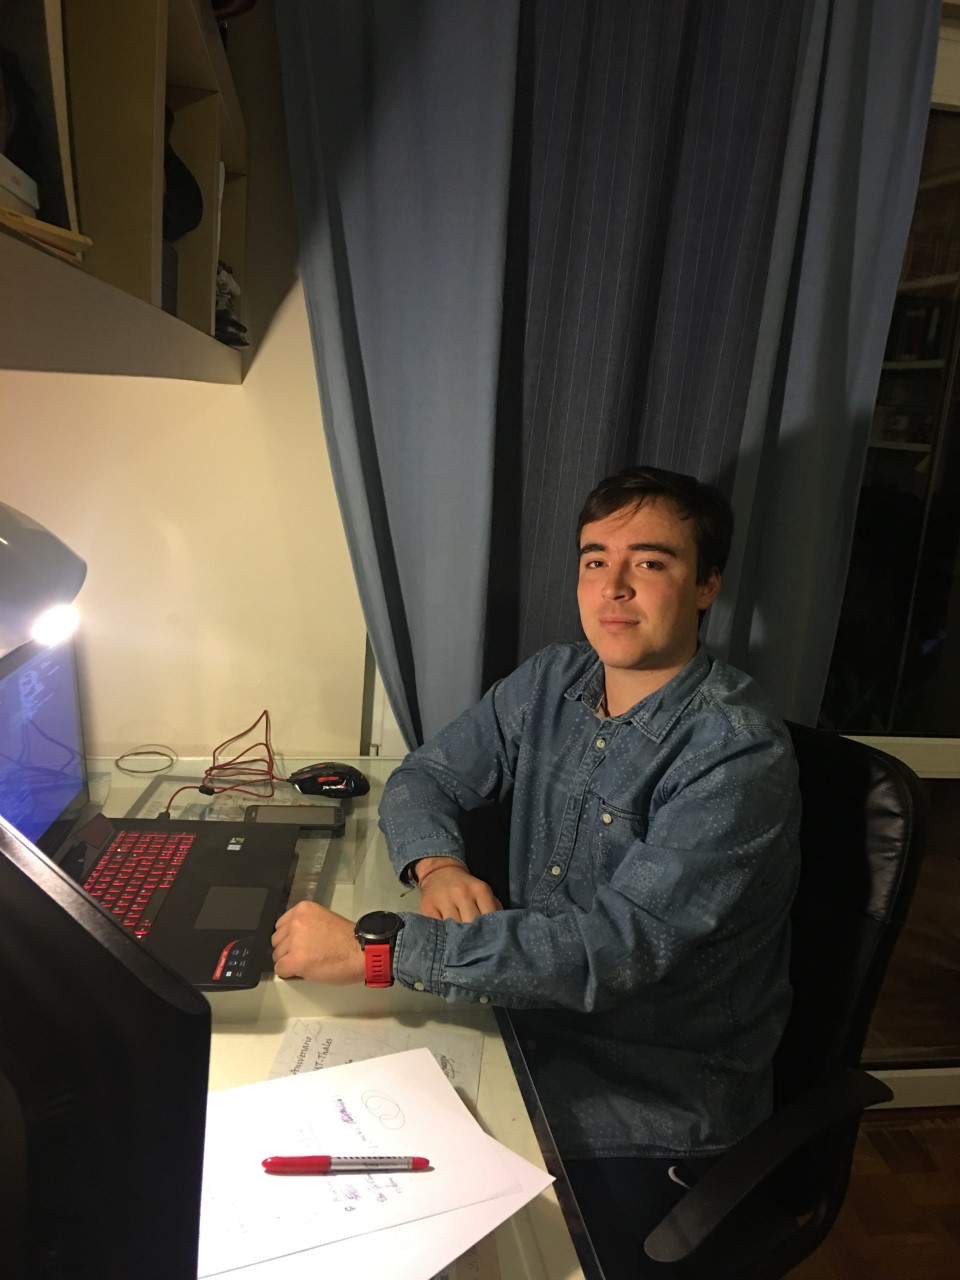
\includegraphics[width=0.6\columnwidth]{Linkedin.jpg}\\[\baselineskip] % Your photo
 		\small % Smaller font size
 		Iván Sevillano García \\ % Your name
 		\url{isega24@hotmail.com} \\ % Your email address
 		\url{github.com/isega24} \\ % Your URL
 		+34 609492713 \\ % Your phone number
 		\Sep % Some whitespace
 		\textbf{Dirección 1} \\
 		C/Buensuceso \\
 		47 2ºI\\ % Address 2
 		18003 Granada \\ % Address 3
 		España \\
 		\textbf{Dirección 2} \\
 		C/Dinamarca, Nº 24 \\ % Address 1
 		Málaga, 29620 \\ % Address 2
 		España \\ % Address 3
 		\vfill % Whitespace under this block to push it up under the photo
 	\end{flushright}
 }
 
 %----------------------------------------------------------------------------------------
 
 \begin{document}
 	
 	\userinformation % Print your information in the left column
 	
 	\framebreak % End of the first column
 	
 	%----------------------------------------------------------------------------------------
 	%	HEADING
 	%----------------------------------------------------------------------------------------
 	
 	\cvheading{Iván Sevillano García} % Large heading - your name
 	
 	\cvsubheading{Ingeniero del Software} % Subheading - your occupation/specialization
 	
 	%----------------------------------------------------------------------------------------
 	%	ABOUT ME
 	%----------------------------------------------------------------------------------------
 	
 	\aboutme{Sobre mi}{}
 	
 	%----------------------------------------------------------------------------------------
 	%	EDUCATION
 	%----------------------------------------------------------------------------------------
 	
 	\CVSection{Educación}
 	
 	%------------------------------------------------
 	
 	\CVItem{2012-201?, Universidad de Granada(UGR)}{Estudios universitarios , Doble Grado en Ingeniería Informática y Matemáticas}
 	
 	\CVItem{Final project}{Clasificación de imágenes de cáncer: Análisis teórico y práctico del
 		aprendizaje profundo.}
 		
 	
 	%------------------------------------------------
 	
 	\CVItem{2016,Universidad de Lodz(Polonia)}{Erasmus+}
 	
 	\CVItem{Languages}
 	{\begin{tabular}{p{0.2\textwidth} p{0.2\textwidth} p{0.2\textwidth}}
 			\bluebullet Español Residente &
 			\bluebullet Inglés(B2)
 		\end{tabular}}
 	
 	%------------------------------------------------
 	
 	\Sep % Extra whitespace after the end of a major section
 	
 	%----------------------------------------------------------------------------------------
 	%	EXPERIENCE
 	%----------------------------------------------------------------------------------------
 	
 	
 	%------------------------------------------------
 	
 	
 	%------------------------------------------------
 	
 	\Sep % Extra whitespace after the end of a major section
 	
 	%----------------------------------------------------------------------------------------
 	%	COMMUNICATION SKILLS
 	%----------------------------------------------------------------------------------------
 	

 	
 	%------------------------------------------------
 	
 	\Sep % Extra whitespace after the end of a major section
 	
 	%----------------------------------------------------------------------------------------
 	%	SKILLS
 	%----------------------------------------------------------------------------------------
 	
 	\CVSection{Habilidades para el desarrollo del Software}
 	
 	%------------------------------------------------
 	
 	\CVItem{Lenguajes de programación}
 	{\begin{tabular}{p{0.2\textwidth} p{0.2\textwidth} p{0.2\textwidth}}
 			\bluebullet Java &  \bluebullet Shell & \bluebullet Python\\
 			\bluebullet C++ &  \bluebullet wxMaxima & \bluebullet Octave\\
 			\bluebullet PHP & \bluebullet MySQL y similares\\
 		\end{tabular}}
 		
 		%------------------------------------------------
 		
 		\CVItem{Entornos de trabajo}
 		{\begin{tabular}{p{0.2\textwidth} p{0.2\textwidth} p{0.2\textwidth}}
 				\bluebullet Github &  \bluebullet Texstudio & \bluebullet Oracle \\
 				\bluebullet Netbeans &  \bluebullet Texstudio & \bluebullet Oracle \\
 			\end{tabular}}
 			
 		\CVItem{Proyectos}{Trabajando y colaborando en algunos proyectos en mi directorio de github\\
 			(https://github.com/isega24).}
 			%------------------------------------------------
 			
 			\Sep % Extra whitespace after the end of a major section
 			
 			%----------------------------------------------------------------------------------------
 			%	NEW PAGE DELIMITER
 			%	Place this block wherever you would like the content of your CV to go onto the next page
 			%----------------------------------------------------------------------------------------
 			
 			\clearpage % Start a new page
 			
 			\userinformation % Print your information in the left column
 			
 			\framebreak % End of the first column
 			
 			%----------------------------------------------------------------------------------------
 			%	AWARDS
 			%----------------------------------------------------------------------------------------
 			
 			\CVSection{Premios}
 			
 			%------------------------------------------------
 			
 			\CVItem{2012, \textit{Matricula de honor}, IES Litoral}{Recompensado en Bachillerato por ser uno de los estudiantes con mejor expediente de ese año.}
 			
 			\CVItem{2006, \textit{Olimpiada matemática Thales}, Andalucía}{Consiguió entrar en el top 5 de los participantes en la Olimpiada en Málaga y pasó a la fase Andaluza.}
 			
 			\CVItem{2007, \textit{Programa ESTALMAT}, Organización ESTALMAT}{Fué parte de los estudiantes acogidos por el Programa del EStimula para el TALento MATematico.}
 			
 			\CVItem{2011, \textit{Olimpiadas matemáticas de Bachillerato}, España }{Participó en las Olimpiadas Matemáticas de Bachillerato.}
 			
 			
 			
 			%------------------------------------------------
 			
 			\Sep % Extra whitespace after the end of a major section
 			
 			%----------------------------------------------------------------------------------------
 			%	INTERESTS
 			%----------------------------------------------------------------------------------------
 			
 			\CVSection{Intereses}
 			
 			%------------------------------------------------
 			
 			\CVItem{Profesional}{Analisis de datos, company profiling, Analisis de riesgo, diseño de Software, automatización de tareas, desarrollo de Inteligencia Artificial, Matemáticas.}
 			
 			%------------------------------------------------
 			
 			\CVItem{Personal}{Guitarra, ajedrez, bailar, running, viajar.}
 			
 			%------------------------------------------------
 			
 			\Sep % Extra whitespace after the end of a major section
 			
 			%----------------------------------------------------------------------------------------
 			
 			%----------------------------------------------------------------------------------------
 			%	CARNET DE COHE
 			%----------------------------------------------------------------------------------------
 			
 			\CVSection{Movilidad}
 			
 			\CVItem{Carnet de coche}{Posesión del carnet B1 de circulación B1 desde Septiembre de 2013.}
\end{document}
 		